% =====================================================================
% Slide 12: Stage 5b -- NN-driven MEAM optimization
%   Left  : training process as bullets + Adam/Huber explained in body
%   Right : training-loss curve + result summary (histogram removed)
% =====================================================================
\begin{frame}{Stage 5b: NN-Driven MEAM Parameter Optimisation}
\fwtag{TensorFlow + LAMMPS}
\begin{columns}[T]
\column{0.5\textwidth}
\textbf{Closed-loop training process}
\begin{enumerate}\scriptsize
  \item \textbf{Surrogate.} A 4-layer MLP
        ($\to\!20\!\to\!20\!\to\!10\to$, ReLU) learns
        $(\text{MEAM params}) \to (C_{11}, C_{12})$.
  \item \textbf{Fit.} Trained with \emph{Adam}~\citep{kingma2015adam}
        on a \emph{Huber} loss ($\delta=1$), up to $10^{4}$ epochs,
        early-stopped once the loss falls below $5\!\times\!10^{-3}$.
  \item \textbf{Inverse step.} Adam (lr $0.01$, $3000$ steps) descends
        through the \emph{frozen} surrogate to the MEAM parameters that
        hit the target $(C_{11}, C_{12})$.
  \item \textbf{Loop.} Optimised parameters are re-evaluated in LAMMPS;
        new samples are appended and the surrogate retrained
        (active learning).
\end{enumerate}

\smallskip
\begin{block}{Why these choices}
\scriptsize
\textbf{Adam} --- adaptive-moment gradient optimiser: per-parameter step
sizes from running gradient moments, a robust default for NN training.\\
\textbf{Huber loss} --- squared-error for small residuals, absolute-error
for large ones; outlier configurations (Mg/Zn) cannot dominate the fit.
\end{block}

\column{0.5\textwidth}
\centering
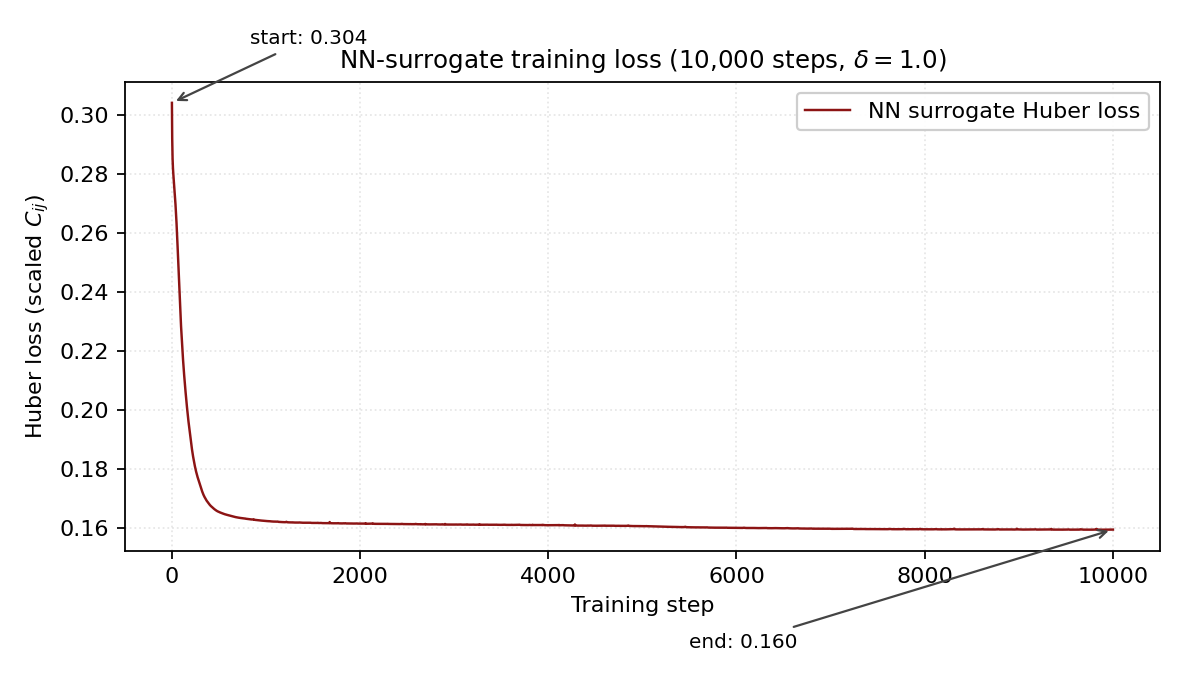
\includegraphics[width=0.74\linewidth]{figures/nnip_training_loss.png}\\[-0.4em]
\scriptsize Surrogate Huber-loss decays $1.0 \to 0.16$ over training.

\smallskip
\begin{block}{Result --- a working proof of concept}
\scriptsize
Tested on \textbf{30 unseen alloys}:
\begin{itemize}\scriptsize
  \item \textbf{11} gave a physically stable potential;
  \item \textbf{4} matched the MD reference within $\sim\!20\,\%$.
\end{itemize}
The pipeline runs end-to-end; accuracy grows with more data and
longer training (next slide).
\end{block}
\end{columns}
\end{frame}
